\documentclass{article}
\usepackage{listings}
\usepackage{graphicx}
\author{Yuxiang Chen 5110309783}
\title{Report of Lab1}
\begin{document}
\maketitle
\tableofcontents
\section{The Purpose of Lab1 and My Preparation}
I think the purpose of lab1 is to give us a primary impression on what html is and how it works.Meanwhile,we also need to learn how to use the BeautifulSoup in parser to get the url of the pictures and some links. So after installing all the softwares we need in the experiment, I spent some time reading the 'parser.pdf' carefully and surfing on the Internet for more information about html and BeautifulSoup, and during which time ,I found that BeautifulSoup is really a good tool to get what we want in the origin codes of a certain  website. Meanwhile, I also tried to write codes in the form of html to make myself understand more. And of course, I also met some trouble, which will be written later.
\section{The Main Part of the Experiment}
\subsection{Exercise 1}
These are my codes about exercise 1:\\
\begin{lstlisting}[language=python,numbers=left,frame=leftline]
def parseURL(content):
    import re
    from BeautifulSoup import BeautifulSoup
    soup=BeautifulSoup(content)
    urlset=set()
    for i in soup.findAll('a',{'href':re.compile('^http*')}):
        urlset.add(i['href'])
    return urlset
\end{lstlisting}
In this part, I use the method given in parser.pdf to find all <a> tag (in order to get rid of the interruption of the url of images) and add each url I found to the set called urlset. Of course, when we execute this program, we need to input some codes to tell the program what 'content' is. \\
So the picture below is a screenshot of exercise 1.\\
\begin{figure}[htbp]
\centering
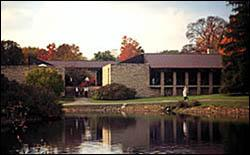
\includegraphics[width=10cm]{1.png}
\caption{the outcome of exercise 1}
\end{figure}
\subsection{Exercise 2}
And the following codes are about exercise2.\\
\begin{lstlisting}[language=python,numbers=left,frame=leftline]
def parseIMG(content):
    import re
    from BeautifulSoup import BeautifulSoup
    soup=BeautifulSoup(content)
    imgset = set()
    for i in soup.findAll('img',{'src':re.compile('^http*')}):
        imgset.add(i['src'])
    return imgset
\end{lstlisting}
And since we only need to get the url of all of the pictures on the website, so it is obvious that we should directly find the links with the tag of 'img'. Then I add all the url I found to the final set named imgset and return the result.\\
Here is the screenshot of excuting the codes in pyscripter.\\
\begin{figure}[htbp]
\centering
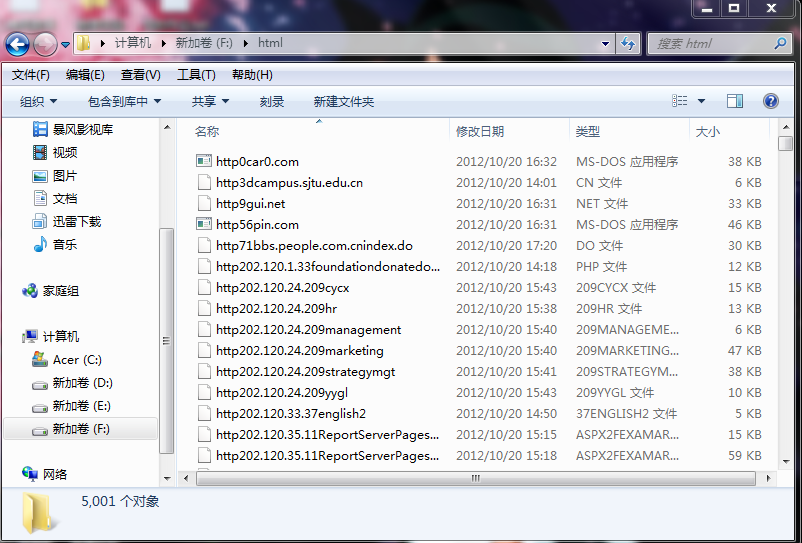
\includegraphics[width=10cm]{2.png}
\caption{the outcome of exercise 2}
\end{figure}
\subsection{Exercise 3}
In the third exercise, we need to return the contents and url of the images of all pictures we find as well as the url of the next page. Comparing to the former two exercise, this exercise is a little harder, but luckily, it's still based on the method we learned in 'parser.pdf'.\\
And here are my codes.\\
\begin{lstlisting}[language=python,numbers=left,frame=leftline]
def parseQiushibaikePic(content):
    import sys
    reload(sys)
    sys.setdefaultencoding('utf8')
    import re
    from BeautifulSoup import BeautifulSoup
    soup=BeautifulSoup(content)
    docs={}
    nextpage=''
    temp=soup.find('div',{'class':'col1'})
    for i in temp.findAll('div',{'class':'block untagged'}):
        docs[i['id']]={}
        for j in i.findAll('div',{'class':'content'}):
            docs[i['id']]['content']=str(j.string).encode('utf8')
        for k in i.findAll('div',{'class':'thumb'}):
            docs[i['id']]['imgurl']=k.find('img')['src']
    for i in soup.findAll('a',{'class':'next'}):
        nextpage='http://www.qiushibaike.com'+i['href']
    return docs,nextpage
\end{lstlisting}
I found that the coded system in python is ascii by default. In order to change it to utf8, which is widely used on most of the websites, I searched on the Internet and found that we can change it by adding these codes before our main program:\\
\begin{lstlisting}[language=python,numbers=left,frame=leftline]
    import sys
    reload(sys)
    sys.setdefaultencoding('utf8')
\end{lstlisting}
And these are also showed in the final codes of exercise3 above. Then I only need to find certain tags to fix the positions of the pictures we need and get the contents and url of them using the same way as exercise1 and exercise2. And there's just one thing left for me to do -- put the information I got in the form of a dictionary.\\
The process and the result are shown in the following two screenshots.\\
\begin{figure}[htbp]
\centering
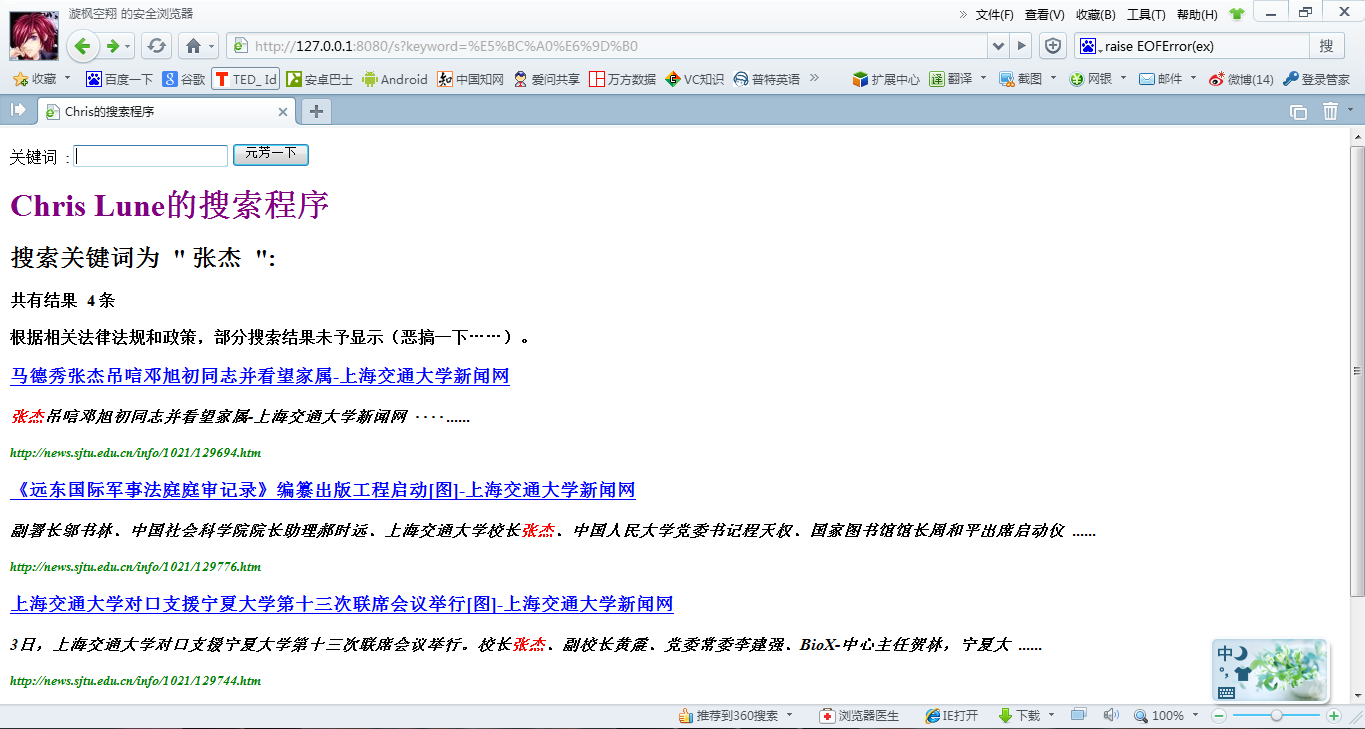
\includegraphics[width=10cm]{3.png}
\caption{the outcome of docs in exercise 3}
\end{figure}
\begin{figure}[htbp]
\centering
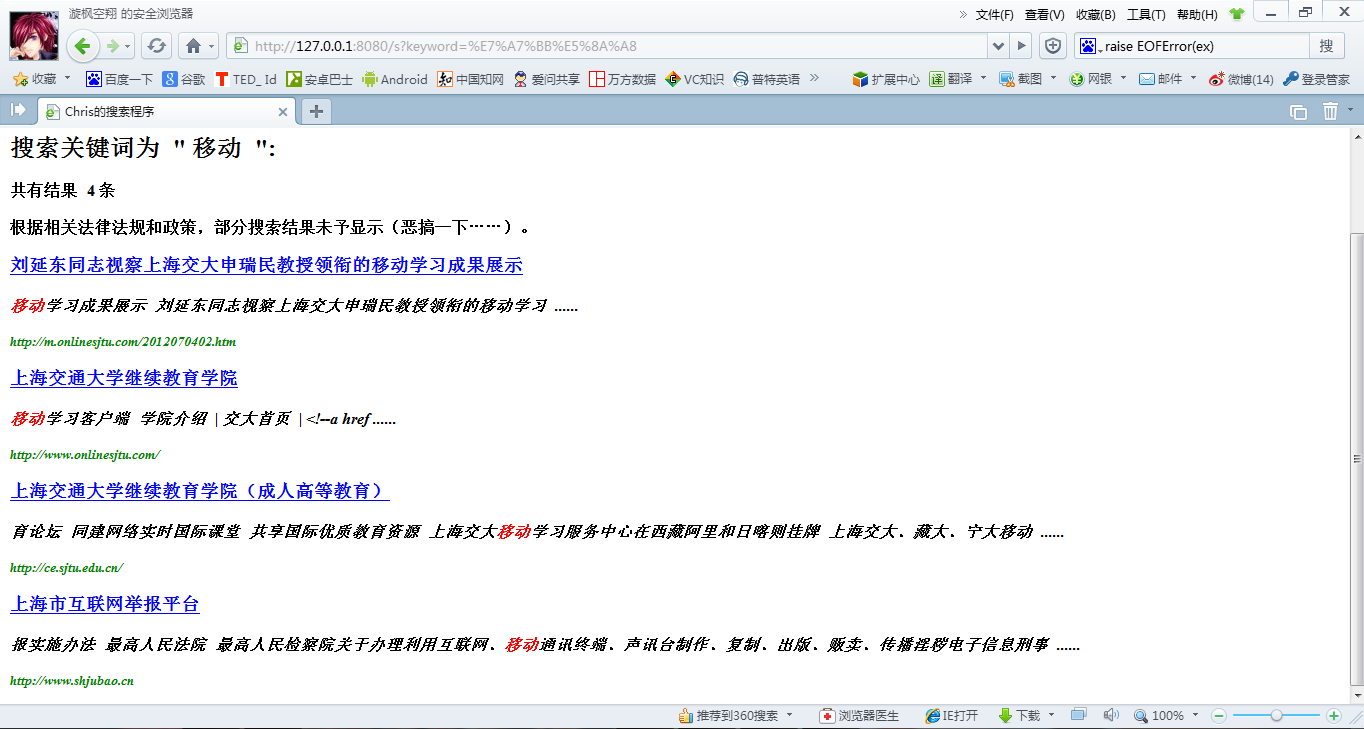
\includegraphics[width=10cm]{4.png}
\caption{the outcome of nextpage and the contents in exercise 3}
\end{figure}
Since the information is too much, so I only show you a small part of the results in the screenshot.
\section{The Problems I Met in the Experiment}
Though the experiment seems really easy, I have to say, it really took me a lot of time to finish it.\\
The first problem is that I have nearly forgot all about the basic knowledges of python, which means I have to review it... Luckily, by searching and reading my old books and notes, I find myself can command it now. \\
The second problem is that in the third exercise, I had some trouble encoding the information in the form of utf8. It is mainly because I didn't remember the defaulting code system in python is ascii, and then I read many essays about it and find the right method to solve the problem, which I have mentioned in the former section. Then it became easy for me to encode the messages. Although in this part, the problem of the encoded mode really drives me mad, I strengthened my understanding about them.
\section{Some of My Thoughts}
Firstly ,I want to say something about the use of the method shown in the experiment in my opinion. I think since we could get the url of the pictures or some links by using BeautifulSoup, maybe we can also get the information hidden by some websites in the form of 'replying to the subjects and then you get the download links', which means it's easier for us to get the information we need without doing other annoying things. Meanwhile, I think we can also find the address of the people leaving messages on the Internet in the anonymous mode, which will contribute to the safety of the network. And after learning what web pages consist of, I think it is now possible for us to set up our own websites. Of course, above are all my thoughts, I can't prove whether they are true now. But I will try to prove them after I learn more.\\
Then I wanna say my own feelings in the experiment. It is an experiment that not only makes me understand more about what 'python' can do, but also remind me of the wonderful function of BeautifulSoup in finding url. And I really learned a lot in the process of searching for some knowledges about them.
\end{document}
